\section{Single Tuned Mass Damper}
\begin{figure}[ht]
    \centering
    % \documentclass[border=1mm, class=article preview]{standalone}
\documentclass[border=5pt,tikz]{standalone}
\usepackage{tikz}
\usetikzlibrary{calc,patterns,decorations.pathmorphing,decorations.markings}

\begin{document}

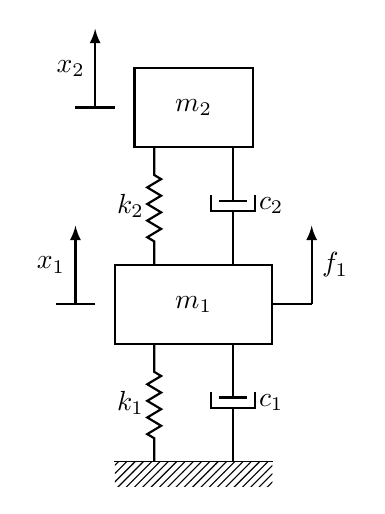
\begin{tikzpicture}
% TikZ Styles
\tikzstyle{mass}=[draw,outer sep=0pt,thick]
\tikzstyle{spring}=[thick,decorate,decoration={zigzag,pre length=0.3cm,post length=0.3cm,segment length=6}]
\tikzstyle{damper}=[thick,decoration={markings,  
  mark connection node=dmp,
  mark=at position 0.5 with 
  {
    \node (dmp) [thick,inner sep=0pt,transform shape,rotate=-90,minimum width=15pt,minimum height=3pt,draw=none] {};
    \draw [thick] ($(dmp.north east)+(2pt,0)$) -- (dmp.south east) -- (dmp.south west) -- ($(dmp.north west)+(2pt,0)$);
    \draw [thick] ($(dmp.north)+(0,-5pt)$) -- ($(dmp.north)+(0,5pt)$);
  }
}, decorate]
\tikzstyle{ground}=[fill,pattern=north east lines,draw=none,minimum width=0.75cm,minimum height=0.3cm]
% Actual Drawing
\node (m2) [mass,minimum width=1.5cm,minimum height=1cm] {$m_2$};
\node (m1) at (m2.south) [mass,yshift=-1.5cm,anchor=north,minimum width=2cm,minimum height=1cm] {$m_1$};
\node (ground) at (m1.south) [ground,yshift=-1.5cm,anchor=north,minimum width=2cm] {};
\draw (ground.north west) -- (ground.north east);
\draw [spring] ([xshift=-0.5cm] ground.north) -- ([xshift=-0.5cm] $(m1.south east)!(ground.north)!(m1.south west)$) node[midway, left]{$k_1$};
\draw [damper] ([xshift=0.5cm] ground.north) -- ([xshift=0.5cm] $(m1.south east)!(ground.north)!(m1.south west)$) node[midway, right,xshift=2mm]{$c_1$};
\draw [spring] (m1.135) -- ($(m2.south east)!(m1.135)!(m2.south west)$) node[midway, left]{$k_2$};
\draw [damper] (m1.45) -- ($(m2.south east)!(m1.45)!(m2.south west)$) node[midway, right,xshift=2mm]{$c_2$};
\draw [thick] (m1.east) -- +(0.5cm,0);
\draw [-latex,thick] ([xshift=0.5cm]m1.east) -- +(0,1cm) node[midway, right]{$f_1$};
\draw [thick] ([xshift=-0.25cm]m1.west) -- +(-0.5cm,0);
\draw [-latex,thick] ([xshift=-0.5cm]m1.west) -- +(0,1cm) node[midway, left]{$x_1$};
\draw [thick] ([xshift=-0.25cm]m2.west) -- +(-0.5cm,0);
\draw [-latex,thick] ([xshift=-0.5cm]m2.west) -- +(0,1cm) node[midway, left]{$x_2$};
\end{tikzpicture}

\end{document}
    \caption{\raggedright SDOF System with STMD}
    \label{fig:STMD}
\end{figure}
The first TMD we would like to analyse is a single tuned mass damper (STMD) attached to $m_1$. The only constraint that we have is $m_2=0.1\,kg$.
\subsection{Analysis}
Equation of motion (EOM) can be written as:
\begin{center}
$$
\begin{bmatrix}
m_1 & 0\\
0 & m_2
\end{bmatrix}\cdot
\begin{Bmatrix}
\ddot{x_1}\\
\ddot{x_2}
\end{Bmatrix}+
\begin{bmatrix}
c_1+c_2 & -c_2\\
-c_2 & c_2
\end{bmatrix}\cdot
\begin{Bmatrix}
\dot{x_1}\\
\dot{x_2}
\end{Bmatrix}+
\begin{bmatrix}
k_1+k_2 & -k_2\\
-k_2 & k_2
\end{bmatrix}\cdot
\begin{Bmatrix}
x_1\\
x_2
\end{Bmatrix} =
\begin{Bmatrix}
f_1\\
0
\end{Bmatrix}
$$
\end{center}
In closed form:
$$
[M] \cdot \{ \ddot{X} \} + [C]  \cdot \{ \dot{X} \} + [K] \cdot \{ X \} =  \{ F \}
$$
Assuming $ \{ X \} = \{ X^* \} e^{i \omega t} $ \& $ \{ F \} = \{ F \} sin(\omega t) = Im \{ \{ F \} e^{i \omega t} \} $, taking Fourier transform of the equation:
$$
[-\omega^2[M] + i \omega [C] + [K])]\cdot \{ X^* \} = \{ F \}
$$
$$
\{ X^* \} = [-\omega^2[M] + i \omega [C] + [K])]^{-1} \{ F \}
$$
By solving this equation for different frequencies, we can get the frequency response of the system for different TMD parameters. Effect of different stiffness and damping coefficients can be seen on figures \ref{fig:effect_of_stiffness} and \ref{fig:effect_of_damping}.
\begin{figure}[ht]
    \centerfloat
    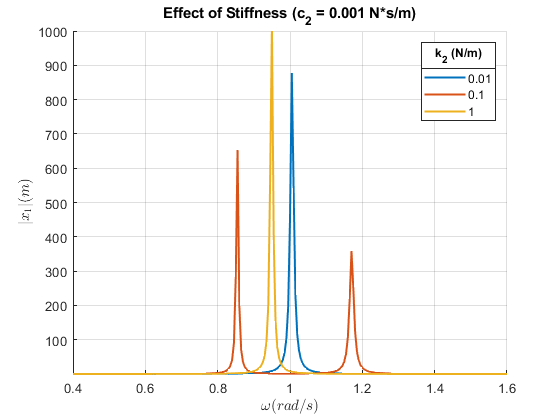
\includegraphics[scale = 0.5]{MATLAB Figures/Effect of Stiffness linear.png}
    \caption{Effect of stiffness variation on STMD}
    \label{fig:effect_of_stiffness}
\end{figure}
\begin{figure}[ht!]
    \centerfloat
    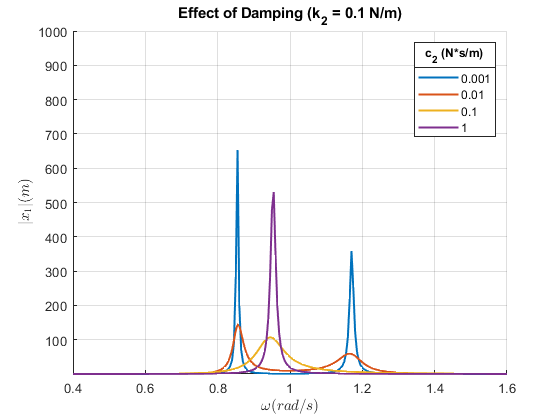
\includegraphics[scale = 0.5]{MATLAB Figures/Effect of Damping linear.png}
    \caption{Effect of damping variation on STMD}
    \label{fig:effect_of_damping}
\end{figure}
\subsection{Optimization}
\par In this configuration of tuned mass damper, we have two parameters ($k_2$ and $c_2$) that need to be changed in order to optimize the response of the system. To find the optimized parameters, we need a quantitative measure of how well a system behaves. The first system measure that can be optimized is the area under the frequency response since area will be reduced as vibrations suppressed further. A gradient base method is used for finding the optimum point. Response of the optimized STMDs can be seen at figure \ref{fig:int_opt_STMD}.
\begin{figure}[ht]
    \centering
    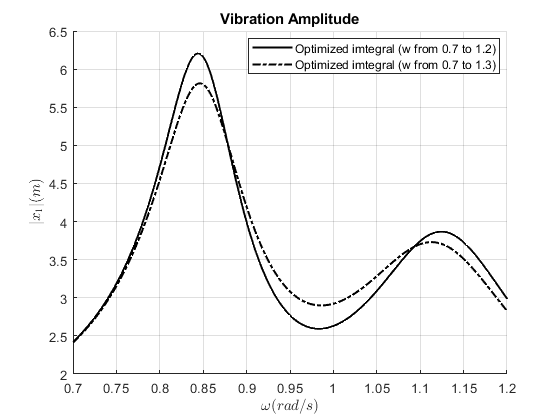
\includegraphics[scale=0.5]{MATLAB Figures/integral_optmized_STMD.png}
    \caption{Frequency response of integral optimized STMDs}
    \label{fig:int_opt_STMD}
\end{figure}
\par
The problem about this method is we can find different optimum values for different bounds of the integral. That prevents us to find the true optimum point. The other system measure that can be used to be optimized is the peak vibration amplitude of the system. To find the peak point, we can use a gradient based optimization technique. As initial guesses, resonance frequencies of undamped system (mode frequencies) can be used. Response of the optimized STMD can be seen at figure \ref{fig:peak_opt_STMD}.
\begin{figure}
    \centering
    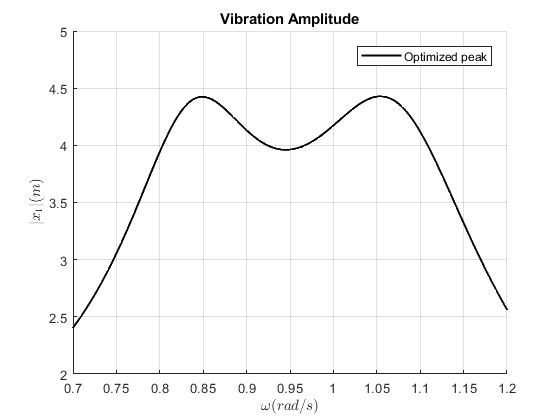
\includegraphics[scale=0.5]{MATLAB Figures/peak_optmized_STMD.png}
    \caption{Frequency response of the peak optimized STMD}
    \label{fig:peak_opt_STMD}
\end{figure}